\section{Datenbanken}


%------------------------------------------------------------------------------
\begin{frame}{Von der Entität zur Entitätsmenge = Logisches Datenmodell Bsp. See}
  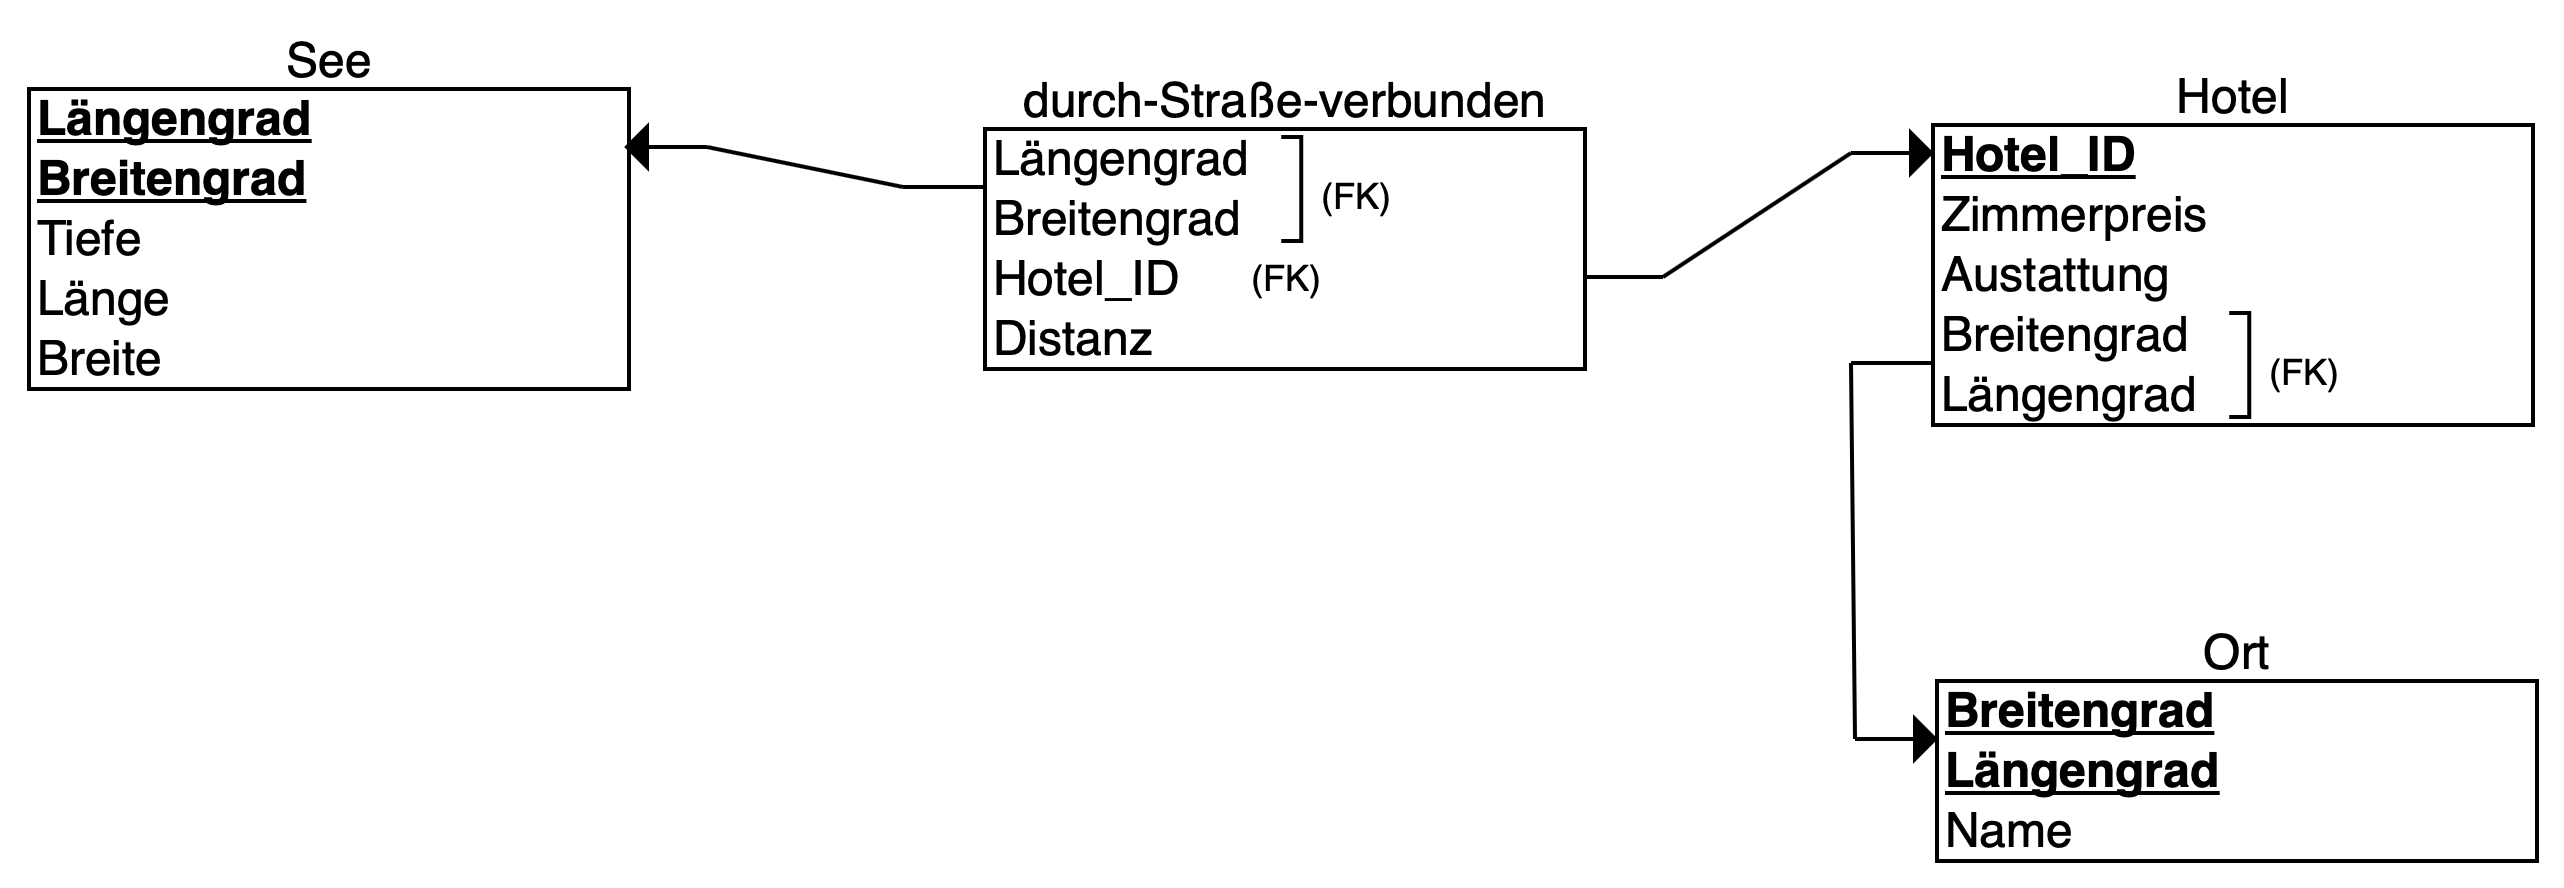
\includegraphics[width=\textwidth]{img/logisches-datenmodell-see.png} 
\end{frame}

%------------------------------------------------------------------------------
\begin{frame}{Datenbank-Schema und Beispiele}
  \metroset{block=fill}
\begin{alertblock}{1) Konzeptionelles Datenmodell}
Entity-Relationship-Diagramm
\end{alertblock}

\begin{alertblock}{2) Logisches Datenmodell }
\begin{itemize}
    \item relationales Schema
    \item hierarchisches Schema, usw.
\end{itemize}
\end{alertblock}

\begin{alertblock}{3) Physisches Datenmodell}
\begin{enumerate}
    \item \textbf{Relationale Datenbank:} SQLite, MySQL, PostgreSQL, Oracle, Microsoft SQL Server
    \item \textbf{Graphdatenbank:} Blazegraph, Neo4j
    \item \textbf{XML-Datenbank:} existdb
\end{enumerate}
\end{alertblock} 
\end{frame}

%------------------------------------------------------------------------------
\begin{frame}{Datenbank-Definitionen}
  \metroset{block=fill}
\begin{block}{Datenbasis}
Sammlung von Daten, die von einem DBMS verwaltet werden (der Datenbestand in
einem Datenbanksystem)
\end{block}

\begin{block}{Datenbankmanagementsystem (DBMS)}
Software zum Verwalten von Datenbanken
\end{block}

\begin{block}{Datenbanksystem}
Ein Datenbankmanagementsystem und die von ihm verwalteten Daten. \\
Umgangssprachlich ist oft das mit dem Begriff `Datenbank' gemeint.
\end{block}

\end{frame}


%------------------------------------------------------------------------------
\begin{frame}[allowframebreaks]{DBMS}
  \metroset{block=fill}
\begin{alertblock}{Was ist ein Datenbankmanagementsystem (DBMS)?}
Ein Datenbankmanagementsystem ist eine Software zum Betrieb von
Datenbanksystemen, also zur Verwaltung von Datenbasen
\end{alertblock}

\begin{exampleblock}{Basisfunktionalität}
\begin{enumerate}
    \item Definition von Datenstrukturen (via Data Definition Language)
    \item Manipulation von Daten (Einfügen, Ändern, Löschen) (via Data Manipulation Language)
    \item Abfrage  eines Datenausschnitts (via Query Language)
    \item Dauerhafte Speicherung der Daten (nicht zwingend bei jeder DB)
\end{enumerate}
\end{exampleblock}


\end{frame}


%------------------------------------------------------------------------------
\begin{frame}{Historische Datenbankmodelle}
Quelle: DB-LV Slides (Gunter Vasold)
  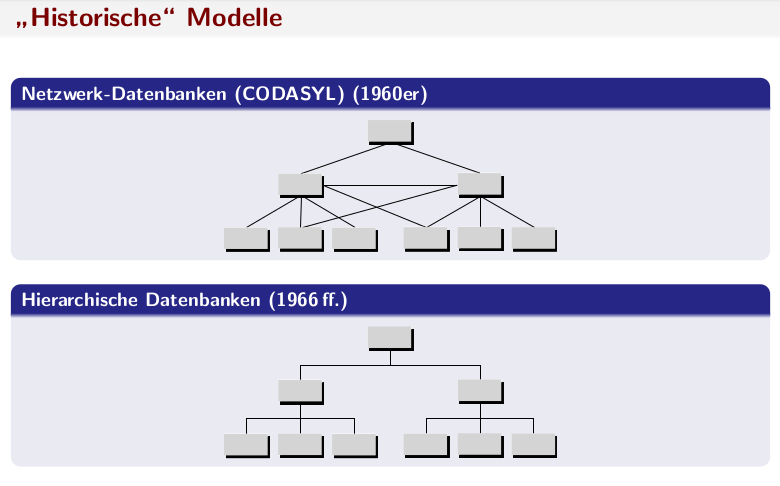
\includegraphics[width=\textwidth]{img/gunther-histor-db-modelle.png}
\end{frame}


%------------------------------------------------------------------------------
\begin{frame}{Relationale Datenbankmodelle}
Quelle: DB-LV Slides (Gunter Vasold)
  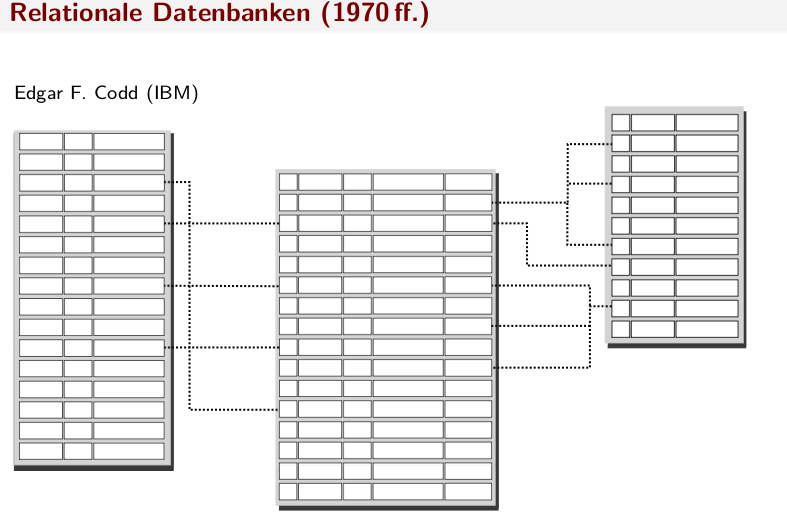
\includegraphics[width=\textwidth]{img/gunter-rel-db.png}
\end{frame}


%------------------------------------------------------------------------------
\begin{frame}{Datenbankmodelle: Historische Entwicklung}
\begin{enumerate}
    \item Objektorientierte Datenbanken (v.a. 1990er-Jahre)
    \item Objektrelationale Datenbanken (1990er-Jahre ff.)
    \item NoSQL-Datenbanken (2000er-Jahre f.)
    \item XML-Datenbanken
    \item Document Stores
    \item Wide Column Stores
    \item Key-Value Stores
    \item Graphenbasierte Datenbanken
\end{enumerate}
\end{frame}


%------------------------------------------------------------------------------
\begin{frame}[standout]
    \alert{Lektüre}-Zusammenfassung: \\
    McCarty, Modelling \\[1em]
    {\footnotesize Bitte \alert{\href{https://docs.google.com/presentation/d/1v_j9Jms21hZokX9hLJ_7kcnV63FJPHTHNowfLVLiYys/edit?usp=sharing}{hier im Google Slides zusammenfassen}}; 1 Person stellt dann vor. \\
    }
\end{frame}


%------------------------------------------------------------------------------
\begin{frame}[standout]
    \alert{Übung:} \\ \small Erklären Sie Ihren Gruppenteilnehmern, welche Entitätstypen in Ihrem Original vorkommen. \\
    Erklären Sie Ihren Gruppenteilnehmern, welchen Zweck ein Filtern und Sortieren der Entitäten für den Modellbenutzer haben könnte.
\end{frame}

